\documentclass[a4paper]{l3proj}
\usepackage{fullpage}
\usepackage{indentfirst}
\usepackage{graphicx}
\usepackage{caption}
\usepackage{subcaption}
\usepackage{enumitem}
\usepackage[usenames,dvipsnames]{xcolor}
\definecolor{customURL}{HTML}{08096E}
\usepackage{hyperref}
\hypersetup{linkcolor=MidnightBlue, urlcolor=customURL, colorlinks}
\def\partautorefname{ }
\def\chapterautorefname{\S}
\def\sectionautorefname{\S}
\def\subsectionautorefname{\S}
\def\subsubsectionautorefname{\S}


\graphicspath{ {images/} }
\begin{document}
\title{A Social Network for Project Task Management}
\author{Gustavo Almansa\\
      Darren Burns \\
      Leonardo Linhares \\
      Euan Parker \\
	  Tom Wallis \\
}
\date{13 October 2014}
\maketitle
\begin{abstract}

The abstract goes here

\end{abstract}
\educationalconsent
\tableofcontents
%============================================================================
\chapter{Introduction}
\label{intro}

%----------------------------------------------------------------------------
\section{Preliminaries}
\label{preliminaries}
A project management tool or suite is a program or set of programs which allows a team of developers, managers, and customers to monitor the state of a project. These tools tend to be used to manage tickets. A ticket is a collection of items of data used to detail a fault, task or feature.  A ticket management system is a type of project management system, whereby it manages and maintains lists of issues documented through tickets. These are notices that members of a development team can set up, discuss code on, and see information about a problem such as its severity and who is responsible for fixing this. Issues and bugs would be found recorded in tickets. They can also hold information about tasks or features that the team has to work on. Records of conversations in ticket comment threads help developers to understand the significance of a ticket, and serve as a platform of discussion on active tickets.


%----------------------------------------------------------------------------
\section{Motivation}
\label{motivation}

A project management tool or suite is a program or set of programs which allow a team of developers, managers, and customers to understand the state of a project. These tools tend to be used to manage tickets. (The act of managing tickets is referred to as ticket management). A ticket is a collection of items of data used to detail a fault, task or feature.  A ticket management system is a type of project management system, whereby it manages and maintains lists of issues documented through tickets. These are notices that members of a development team can set up, discuss code on, and see information about a problem such as its severity and who is responsible for fixing this. Issues and bugs would be found recorded in tickets. They can also hold information about tasks or features that the team has to work on. Records of conversations in ticket comment threads help developers to understand the significance of a ticket, and serve as a platform of discussion on active tickets.


%----------------------------------------------------------------------------
\section{Aims}
\label{aims}

The primary objective of the project was to eliminate redundancy in discussing tickets. The proposition was to create a web-based package where project managers, developers, and customers can discuss a project in a social-networking oriented way. Using conversations, this project should then develop tickets as the conversations being had with calculable and attachable metadata. With appropriate user interface design, using conversations as tickets should solve the three issues laid out in the Motivation section:

\begin{itemize}
\item The project allows for discussion of the issues and bugs within their project management suite.
\item Because discussion occurs directly within a ticket, there is no need to duplicate work as there would be creating tickets on the basis of Skype or Facebook conversations.
\item An easy-to-use user interface would allow for easy ticket management, meaning that the tool would be convenient enough that tickets would get created in the first place.
\end{itemize}

This can result in improved productivity and more thorough documentation of issues.






%----------------------------------------------------------------------------
\section{Outline}
\label{outline}

The dissertation will discuss what was done during the process of developing the system.

\textbf{Initial Planning} \autoref{initialPlanning}

This section discusses how the requirements of the system were developed, and how using this user stories, a user interface mockup and an ER diagram for our system were developed.

\textbf{Implementation} \autoref{impl}

An overview of the process of implementing the system, detailing the creation of different components of the system such as interface, chat system and model layer, as well as how the project progressed over time.

\textbf{Evaluation} \autoref{evaluation}

How the project was evaluated.  This will detail the results of the dogfooding, peer evaluation from another team using the system, and improvements to the system that were identified from this feedback.

\textbf{Conclusion} \autoref{conclusion}

This will detail the current state of the system, whether the aims of the project were achieved, and potential future work that could be done on the system.

%============================================================================

\chapter{Research}
\label{research}
%----------------------------------------------------------------------------
\section{Existing Systems}
\label{existingSystems}

Numerous systems have been created or theorised about which aim to ease or even reinvent the way which software projects are managed.


%----------------------------------------------------------------------------
\subsection{Bugzilla}
\label{bugzilla}

Bugzilla is a bug tracker and testing tool created and used by Mozilla. It integrates with several version control systems such as Git and SVN.  Some interesting features include automated reminders, whereby when bugs are reported but left unresolved the system can be configured to send regular emails to specific people informing them of these bugs. This system is known as the ``whine'' system.  When any change is made to a known bug, this change is added to an automated bug report.  Bugzilla integrates with e-mail, whereby these reports can be e-mailed to the user. Although comparatively simple to use, criticisms of Bugzilla have been made that it is hard to manage errors and there exist many bugs in the program itself.

%----------------------------------------------------------------------------
\subsection{Jira}
\label{jira}
JIRA is a well-used tool for project management, made by Atlassian. Atlassian have a history of working with various aspects of project management, and JIRA integrates with many of these to produce a coherent management environment. However, this makes JIRA less useful on its own, and so there is an identifiable need for a standalone solution, too. Many users of JIRA complain of its difficulty to use, and say that it can be a burdensome way to manage their projects.


%----------------------------------------------------------------------------
\subsection{Asana}
\label{asana}

The unique selling proposition offered by Asana is effective task management without reliance on email. However, the web interface it offers is difficult to understand, and thus results in a large learning curve. Asana also lacks a real-time communication system, relying on comments on tasks for users to communicate. Whilst analysing this product it was found that relying on commenting rather than instant messaging resulted in a lack of urgency, and users were not as inclined to immediately respond. Consequently, users may choose to rely on an external messaging system for communication.

%----------------------------------------------------------------------------
\subsection{Trello}
\label{trello}

Trello is a web-based task management platform which employs the Japanese ``Kanban''
system, originally developed by Toyota. Kanban uses a hierarchical system of
cards, contained within lists, which themselves are contained within boards, to
manage how projects are managed. Kanban is often used to understand the flow of data within the real world, such as in supermarket production lines or in law cases, but also in project management using Trello.

The team used Trello in the early stages of the project before eventually migrating to use the project itself.

%----------------------------------------------------------------------------
\subsection{Producteev}
\label{producteev}

Producteev provides a feature set similar to the aforementioned products, but allows skilled users to quickly navigate the system using numerous shortcuts. A critical feature of Producteev is the ability to convert an email into a task using a Microsoft Outlook extension, thus allowing users to create tasks without have to repeat themselves. This feature is of particular interest to the team, since it... 


%----------------------------------------------------------------------------
\subsection{Slack}
\label{slack}
Slack is an instant messaging system focussed around project management. It can be used in any team-based project, but excels at the management of software projects due to the large number of integrations with external services such as GitHub. Despite Slack not providing a mechanism for directly attaching project related issues to conversations, it was decided that the excellent messaging functionality it provides is something that the project should aim to emulate.

%----------------------------------------------------------------------------
\subsection{Codebook}
\label{codebook}
Codebook was a project management system theorised by Microsoft to visualise the connections between people and their software projects. The project failed to become a public product, but should be noted due to its high degree of social networking and understanding of metadata.

Codebooks most significant lacking in reference to this project’s goals was ticket management. It was not possible to manage a project entirely through Codebook, because it had no ticket management or communication between groups of people; instead, Codebook mapped out projects so workflows could be better understood.

Codebook was never a project that was released to the public, but Microsoft published several papers on it.


%============================================================================
\chapter{Initial Planning}
\label{initialPlanning}

%----------------------------------------------------------------------------
\section{Requirements}
\label{requirements}

The problem that the project aims to solve was established in the initial meetings with the project supervisor. However, developing a set of requirements which would implement a solution for this problem proved more difficult. One of the primary aims of this project is to realise a system which would reduce the duplication of effort that is often required when managing tickets: a team discusses an issue or bug on one platform, and then logs the result in a ticket. This is a problem that existing solutions often make very little or no attempt to solve. Whilst carrying out analysis of existing products and ideas, it was found that Producteev and Codebook attempt to minimise the effects of this issue, and the other systems choose to ignore it completely.

Codebook attempted to solve this problem by closely integrating a social network with software project artifacts. The social network aspect of Codebook was noted by the team as one that may encourage users to use the system both as their primary communication method, and as their project management tool. It was also identified that by giving the software access to tickets and the discussions related to them, a wealth of additional data is available to the system which would otherwise have to be manually entered by a user.

The approach taken by Producteev on the other hand, is to attempt to reduce duplication of effort by allowing users to convert emails into tasks. By allowing users to create a task in this way, we are overcoming the need to copy the information from the email to the task manually.

Both of these features helped inspire the primary requirements of the software. It was deemed a vital requirement that the software tightly integrate social features in order to make use of the data generated through users communicating with each other. In addition, the team decided that the software needed to use this data in order to minimise the effort required in managing a software project. Agile software development aims to prioritise interactions over process, and so the software must be constructed to maintain some degree of process without overly interfering with communication.

Several different ideas for the development of the system were discussed. One suggested approach was that an existing product be extended to attempt to meet the requirements. Suggestions for implementing this approach included:

\begin{itemize}
\item \textit{Interfacing a custom ticket management system with Skype}. \par This approach was rejected due to the lack of control that the Skype API gives with regards to accessing data contained within conversations.
\item \textit{Creating an instant messaging extension for Jira}. \par This approach was rejected due to the emphasis that Jira places on the ticket based approach. Although the required design would have to maintain aspects of this approach, it would have been difficult to focus on communication when there is a major dependence on a colossal, process reliant ticket management system.

\item \textit{Creating an instant messaging extension for Jira}. \par This approach was rejected due to the emphasis that Jira places on the ticket based approach. Although the required design would have to maintain aspects of this approach, it would have been difficult to focus on communication when there is a major dependence on a colossal, process reliant ticket management system.

\end{itemize}

With none of these approaches offering the desired flexibility, it was decided to build the system using Django, a Python web development framework.  As a result of this decision, and in addition to the extensive research of existing project management systems, an initial set of user stories were developed.

%----------------------------------------------------------------------------
\section{User Stories}
\label{userStories}

Listed below is the collection of user stories that were initially created for the system.  Over time these were added to, modified and removed depending various decisions regarding development of the system.

\begin{enumerate}[ref=\arabic*]
\item As a \textit{user} I want to \textit{create an account} on the system so that I can \textit{use the features it offers}. \label{item:1}
\item As a \textit{user} I want to \textit{create a conversation with another user} so that I can \textit{discuss a proposed change}. \label{item:2}
\item As a \textit{project manager} I want to \textit{change other users privileges} so that \textit{I limit other users access}. \label{item:3}
\item  a \textit{developer} I want to \textit{tag a conversation as a ticket} so that \textit{it becomes managed}.\label{item:4}
\item As a \textit{developer} I want to \textit{attach additional meta-data to a ticket} to allow me to keep track of priority, progress and other issues.\label{item:5}
\item As a \textit{developer} I want to \textit{end a conversation or ticket} so that I\textit{don't have to look at irrelevant tickets}.\label{item6}
\item As a \textit{developer} I want to \textit{be able to change priorities of my tickets} so that \textit{more important tasks get priority}.\label{item:7}
\item As a \textit{QA manager} I want to \textit{be able to change the priorities of other peoples tickets} so that I can \textit{decide the importance of certain tasks}.\label{item:8}
\item As a \textit{developer} I want to \textit{assign milestones to a conversation} so that I can \textit{track project velocity}.\label{item:9}
\item As a \textit{developer} I want to \textit{split a conversation} so that I can \textit{separate multiple issues if they appear in a single ticket}.\label{item:10}
\item As a \textit{user} I want to \textit{tag another user} to \textit{add them to a discussion}.\label{item:11}
\item As a \textit{project manager} I want to \textit{view metrics that have been extracted from a ticket} so that I can \textit{monitor my teams progress on an issue}.\label{item:12}
\item As a \textit{developer} I want to \textit{link to a version control repository} so that I can \textit{quickly access the technical side of the ticket}.\label{item:13}
\item As a \textit{user} I want to \textit{attach multimedia to a conversation or ticket} so that I can \textit{explain problems or ideas more easily}.\label{item:14}
\item As a \textit{developer} I want to \textit{assign resolution to an owner} so that it will get done.\label{item:15}
\item As a \textit{user} I want to \textit{add other people to help resolve the issue}.\label{item:16}
\item As a \textit{user} I want to \textit{be able to autocomplete names of other users} so that I can \textit{tag other users correctly and quickly}.\label{item:17}
\item As a \textit{user} I want to \textit{create labels} so that I can \textit{cross reference other conversations}.\label{item:18}
\item As a \textit{developer} I want to \textit{view previous tickets} so that I can \textit{view what has been changed previously}.\label{item:19}
\item As a \textit{project manager} I want to \textit{track the activity of other users} so that I \textit{know what is happening in the project}.\label{item:20}
\item As a \textit{user} I want to \textit{search the website} so that I can \textit{find things within the site quickly}.\label{item:21}
\end{enumerate}

From these user stories a set of high, medium and low priority tasks were determined. The high priority user stories were: \ref{item:1}, \ref{item:2}, \ref{item:5}, \ref{item:7}, \ref{item:12}, \ref{item:19}. Medium priority: \ref{item:11}, \ref{item:15}, \ref{item:18}. Low priority: \ref{item:10}, \ref{item:13}, \ref{item:14}, \ref{item:17}.

\iffalse
\subsection{High Priority}
\begin{itemize}
\item \textit{Create an account} \par
The first page a user should see when loading the website must be a page asking them to log in, or create a new account if they have not already done so.
\item \textit{Create a conversation} \par
There must be a way to create a new conversation to discuss different topics relating to the project.
\item \textit{Create a project} \par
There must be a way to create a new project to manage within the software. 
\item \textit{Add metadata to a conversation} \par
Users must be able to attach relevant metadata to conversations.  Attaching additional information to a chat system is crucial in achieving the goal of combining a ticketing system with social networking.
\item \textit{Change priority of conversations} \par
A user must be able to change the priority of a conversation so that high priority tasks get more attention.  This goes hand-in-hand with adding metadata, whereby priority could be represented as a metadata object.
\item \textit{View previous closed conversations} \par
Viewing previous conversations is essential in seeing what has been achieved so far over the course of a project's lifespan.
\item \textit{View visualisations based on data extracted from conversations} \par
Viewing visual representations of different aspects of a project allows users to determine how much effort is being devoted to a project, how many people are working on a project and each users individual contribution.
\end{itemize}
\subsection{Medium Priority}
\begin{itemize}
\item \textit{Assign resolution of a conversation to an owner} \par
Users should be able to assign a conversation to another user in order to regulate who works on what issue.  This prevents multiple people working on the same thing while another task goes undone.
\item \textit{Tagging other users in a conversation to bring it to their attention} \par
Users should be able to tag other users in a conversation, so that when the subject being discussed relates to.
\item \textit{Linking to other conversations to cross reference discussions} \par
In the event that multiple conversations have a common topic there should be a way to link these conversations, as this allows users to quickly find relevant information pertaining to the topic.
\item \textit{Filtering conversations} \par
Users should be able to filter conversations by typing text for which to search for, and remove any conversations that do not contain these terms.
\item \textit{Saving messages within chats} \par
Users should be able to save messages within chats, so that messages that contain important messages or links can be quickly found.

\end{itemize}
\subsection{Low Priority}
\begin{itemize}
\item \textit{Linking to version control repository} \par
Users could be able to link to version control, so that it is quicker for teams to navigate between different tools relating to the management of the project.

\item \textit{Attach multimedia to a conversation} \par
Attaching media to a conversation could be useful as users may wish to link videos, images or sound clips containing relevant information.

\item \textit{Autocomplete names of users} \par
Autocompleting user names can make it easier to tag other users by ensuring their name is correctly typed.

\item \textit{Branching conversations to separate different issues} \par
Branching conversations could be useful as it allows a discussion that involves multiple topics to be split up into separate conversations, allowing users to only read through information that is relevant.

\end{itemize}

\fi


%----------------------------------------------------------------------------
\section{Design}
\label{design}

Once the initial design goals were established an entity-relationship (ER) diagram was developed for the system. After several iterations, the diagram shown in \autoref{figure:ERDiagram1} was produced. This was used to assist the development by identifying the crucial components of the system. Additionally, the ER diagram greatly assisted in the modelling of our data using the Django Object Relational Mapper, since there is a close correlation between the features of the diagram and the structure of data models in Django.

Due to the experimental nature of the project, rapidly changing requirements meant that that the final model of the system varies from the design in the diagram.

Next, a series of paper based prototypes were created in order to plan the user interface. Paper prototyping was used due to the quick, easy and inexpensive nature whereby multiple different possible designs can be quickly produced and contrasted. Several initial designs were brainstormed. The clutter, intuitiveness and overall appeal of different designs were compared.  An example of different designs that were considered are shown below.

\begin{figure}
\centering
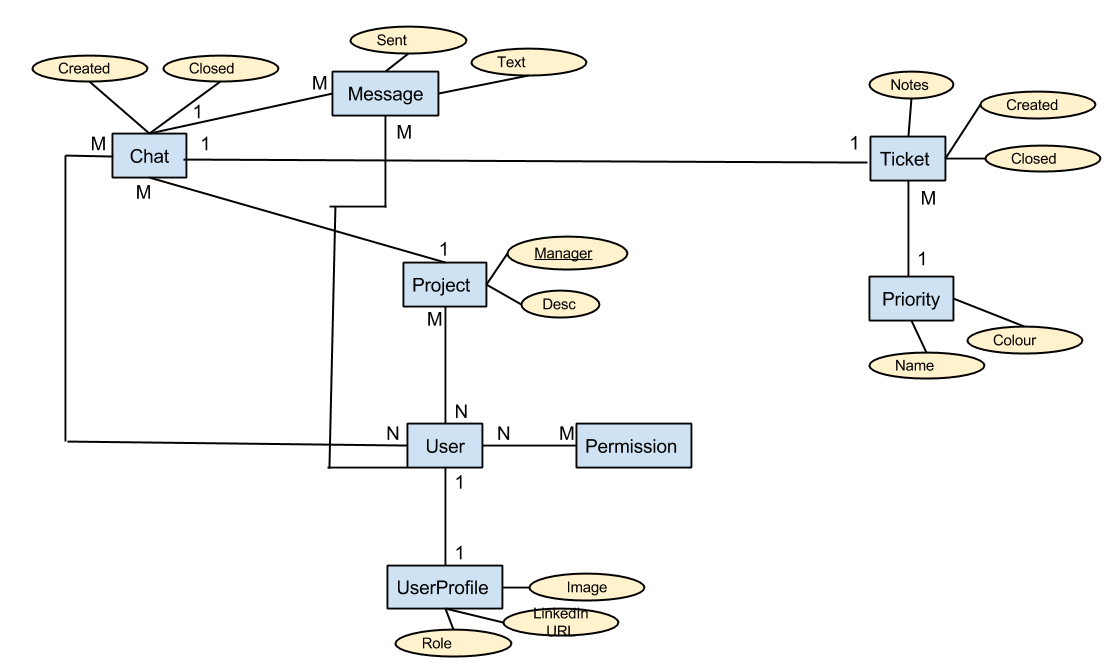
\includegraphics[scale=0.4]{ER_Diagram}
\caption{ER Diagram}
\label{figure:ERDiagram1}
\end{figure} 

\begin{figure}
    \centering
    \begin{subfigure}[b]{0.3\textwidth}
	    \centering
		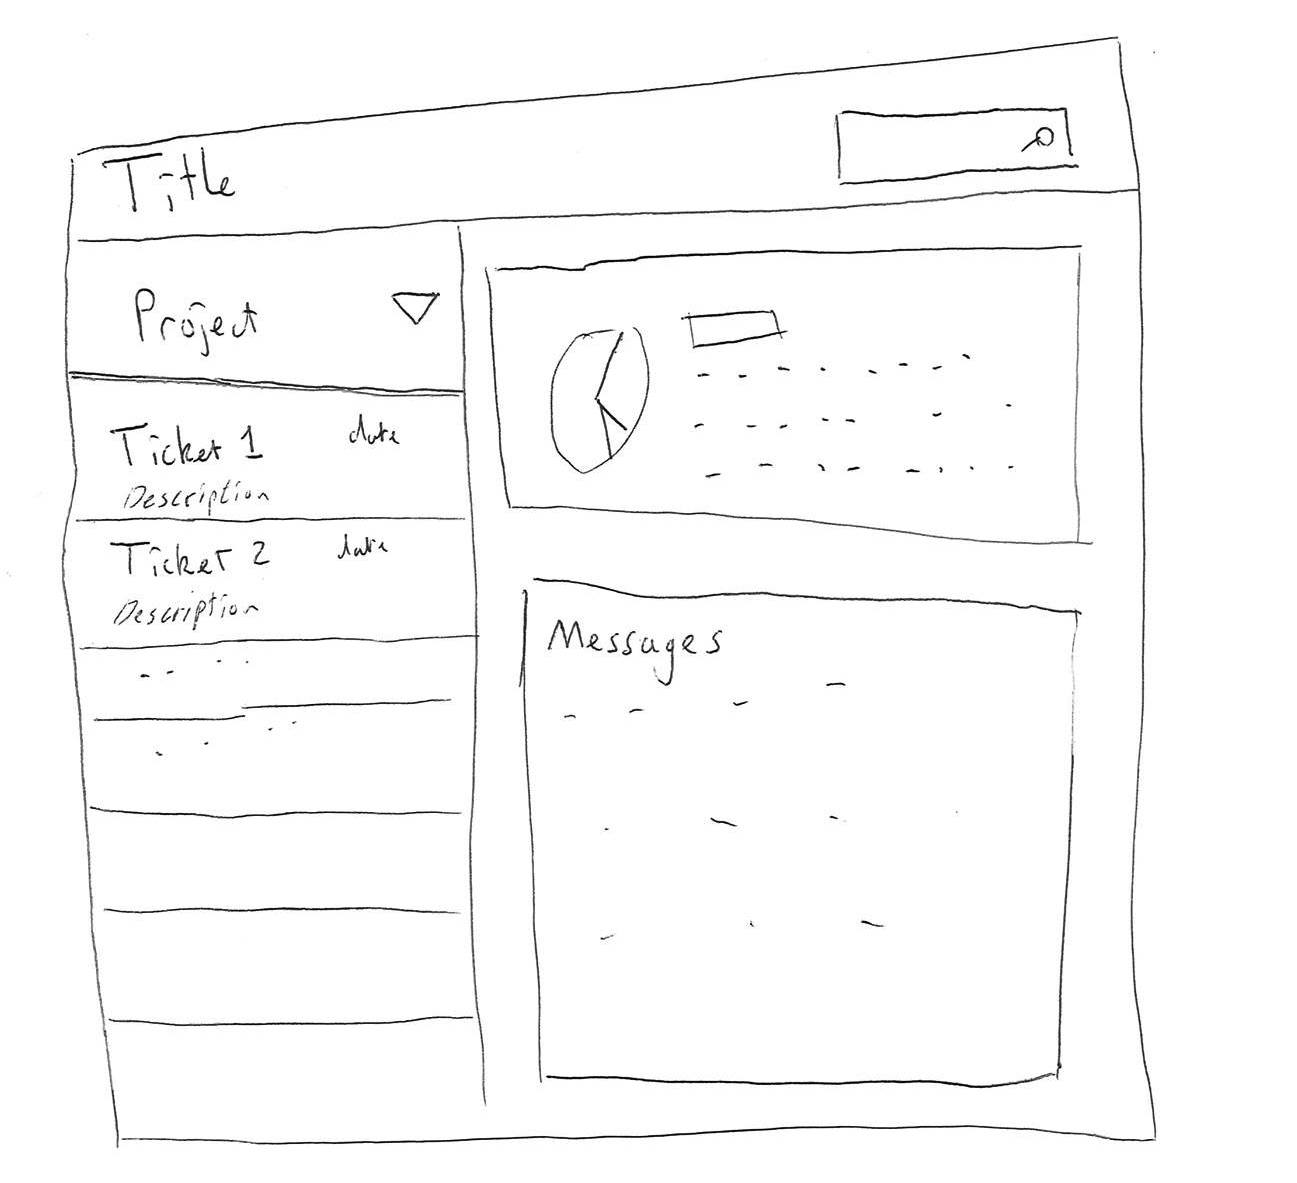
\includegraphics[width=\textwidth]{mockup1}
		\caption{Mockup 1}
		\label{fig:mockup1}        
    \end{subfigure}
    \hfill
    \begin{subfigure}[b]{0.3\textwidth}
        \centering
		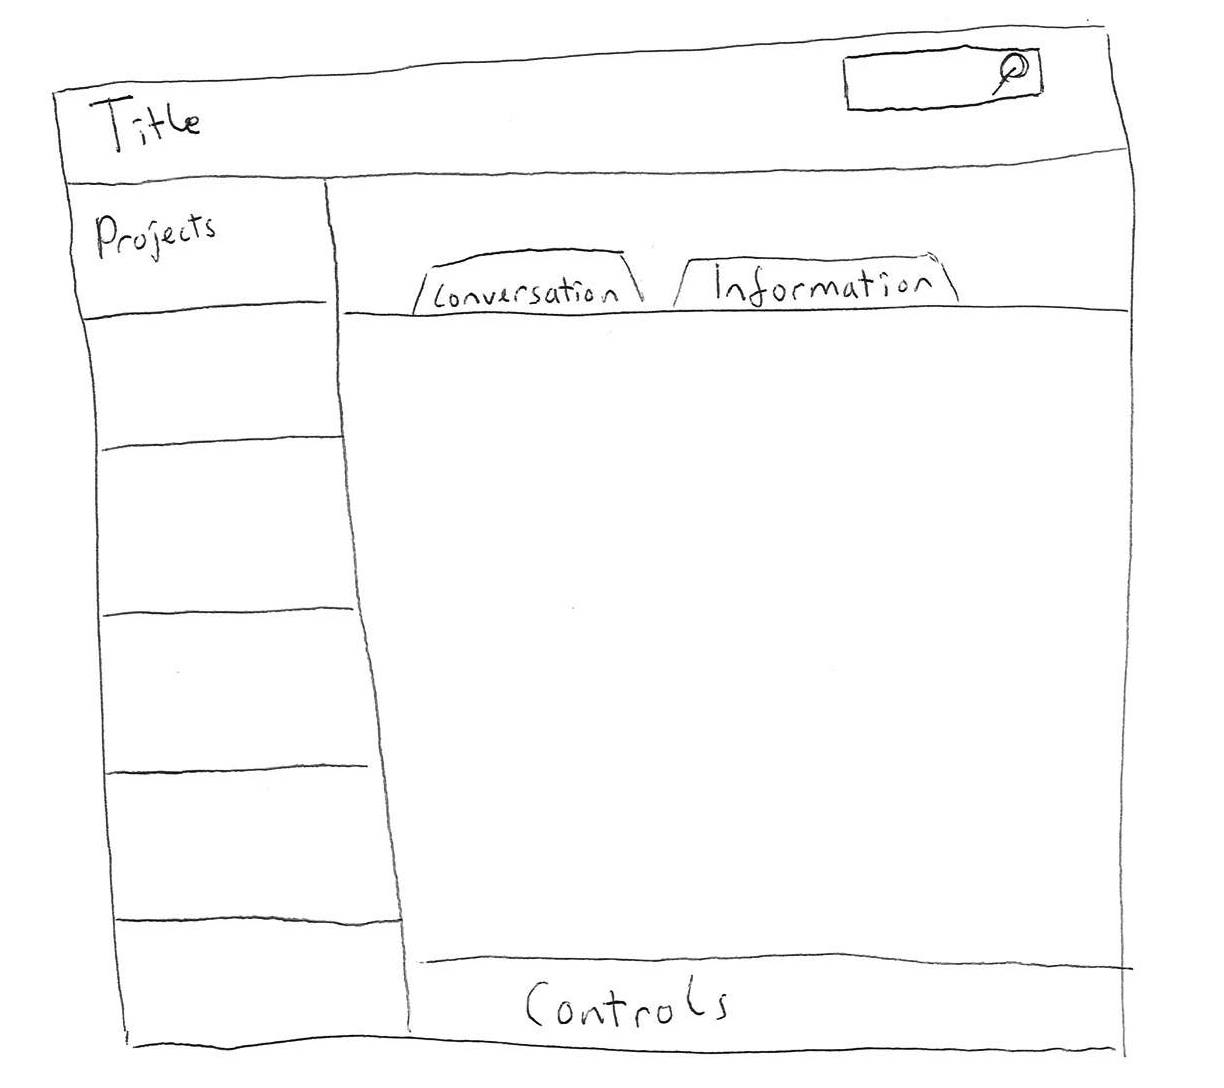
\includegraphics[width=\textwidth]{mockup2}
		\caption{Mockup 2}
		\label{fig:mockup2} 
    \end{subfigure}
    \hfill
    \begin{subfigure}[b]{0.3\textwidth}
        \centering
		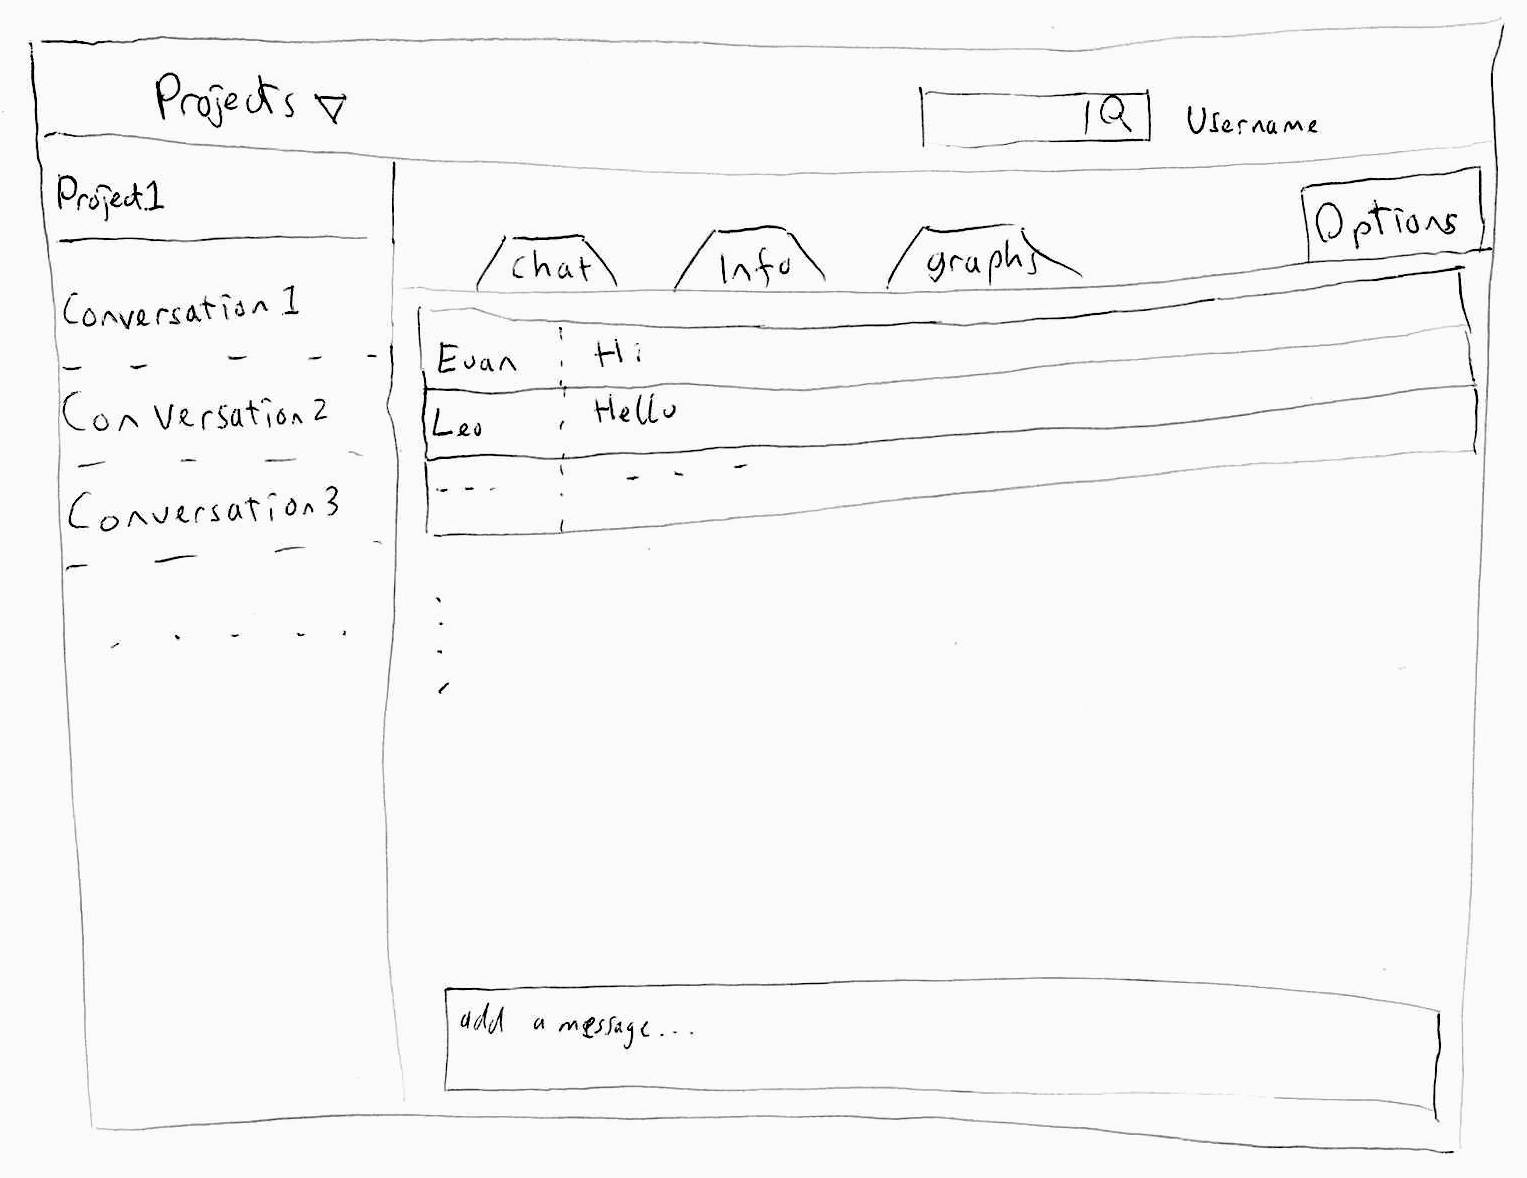
\includegraphics[width=\textwidth]{mockup3}
		\caption{Mockup 3}
		\label{fig:mockup3} 
    \end{subfigure}
    \caption{Three mockups}
    \label{fig:Three mockups}
\end{figure}

\autoref{fig:mockup1} shows the initial prototype for the design, which displayed visualisations relating to the project on the main page.  A project was chosen from a dropdown menu and all the tickets related to that project were listed below.  Each ticket consisted of the graphs,metadata and all the messages for the project.

In \autoref{fig:mockup2}, the ticket appearance was changed whereby the information section was removed and two tabs were added, a ‘conversation’ tab which was used to display the messages, and an ‘information’ tab which displayed visualisations and metadata related to the project. This change was made to reduce clutter in the interface and  A controls section was added which would be used to add new metadata such as due date, priority, assignee etc.

The final design, \autoref{fig:mockup3}, moved the projects drop-down menu into the navbar, with the selected project shown below alongside the relevant conversations.  The controls section was removed and an options menu was added above the conversations.  The information tab was divided into an info and graphs tab, whereby info contained metadata relating to the conversation and graphs contained the visualisations that had been generated with the data.
% The initial prototype for the design displayed visualisations relating to the project on the main page.  A project was chosen from a dropdown menu and all the tickets for the project were listed below.  Each ticket consisted of the graphs,metadata and all the messages for the project.

% In this later version, the ticket appearance was changed whereby the information section was removed and two tabs were added, a ``conversation'' tab which was used to display the messages, and an ‘information’ tab which displayed visualisations and metadata related to the project.  A controls section was added which would be used to add new metadata such as due date, priority, assignee etc.


%----------------------------------------------------------------------------
% \section{Entity Relationship Diagrams}


%============================================================================
\chapter{Team Organisation}
\label{team}

Trello was chosen as the team’s initial task management software, with the intent to swap to the tool being developed when the project had advanced sufficiently, through a process called ‘dogfooding’ whereby the system can be internally evaluated by the team during development. (TODO link to the dogfooding section?)  Facebook chat was used to communicate and arrange meetings.  This split of organisation between Facebook and Trello frustrated some team members which further reinforced the aim of the project - bypassing the repetition of certain tasks over different tools. 


%----------------------------------------------------------------------------
\section{Version Control}
\label{versionControl}

The team elected to use Git as the version control system to manage changes in the source code of the software. Git was used due to multiple team members being familiar with it, and for the integration it has with Github. Making use of version control was vital during development of the project, since features were often being developed simultaneously.

The team maintained two main branches within the Git repository. The master branch, which contained the most stable build, and the beta branch, which was used as a deployment staging area for new features. Some code modifications may work as intended in a development environment and then break when deployed. To overcome this risk, code was first deployed to the beta branch before being merged into the master branch.

One aspect of version control in which the team was eventually diligent in applying was continuous integration, in which feature branches are regularly merged into the master branch. Using continuous integration meant that the live version of the project never strayed too far from the overall set of features that were being developed at a given time. 

Frequent merging of feature branches also provided the added benefit that breaking changes were easier to find, due to the fact that less code was being added in each merge. During the initial stages of the project, branches often went unmerged for several weeks, making integration of features exceptionally difficult. 

After realising the difficulties this workflow caused, this flaw was amended by substantially increasing the rate at which features were merged with the master branch. The diagram \ref{figure:diagram1} shows how features were frequently merged into the master branch (shown as the black line at the top of the diagram) during the week of March 1st 2015.

For comparison, the lack of feature branch integration displayed during the early stages of the project is displayed on diagram \ref{figure:diagram2}. This diagram shows branching activity between the 24th and 30th of November 2014. 

\begin{figure}[ht, ref={\alph}]
\centering
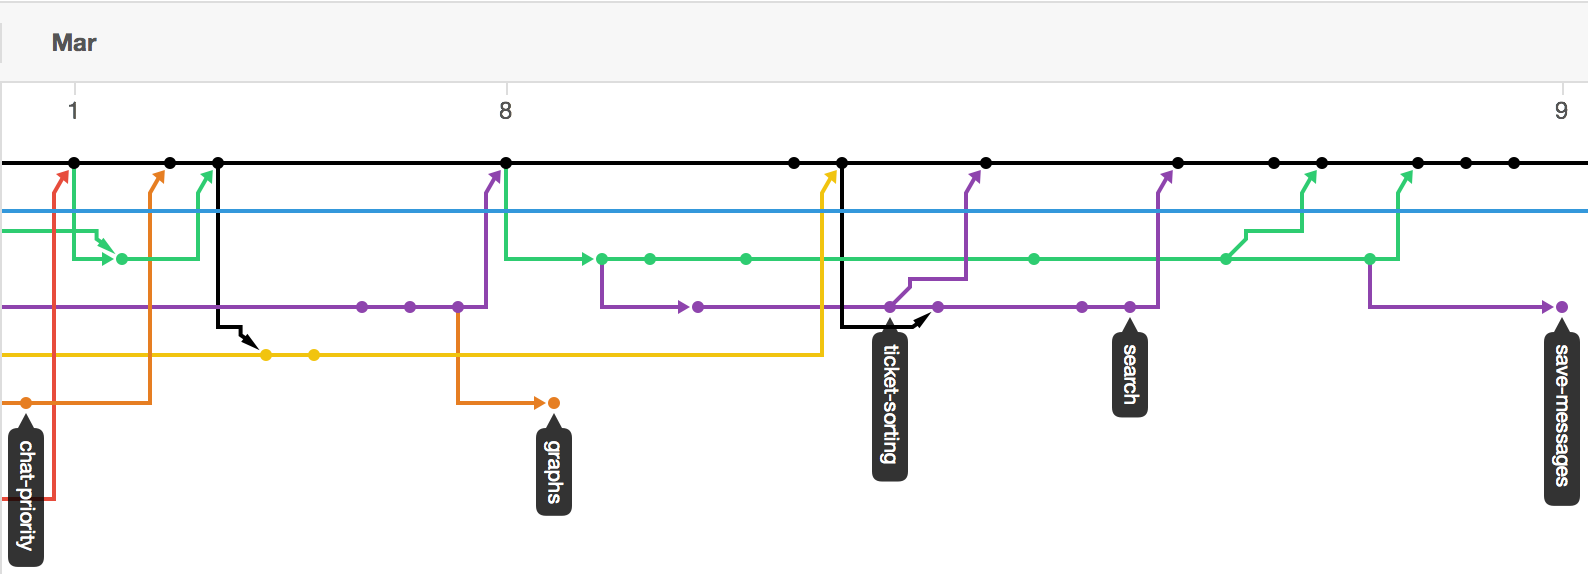
\includegraphics[scale=0.5]{diagram}
\caption{Git diagram 1}
\label{figure:diagram1}
\end{figure} 

\begin{figure}[ht, ref={\alph}]
\centering
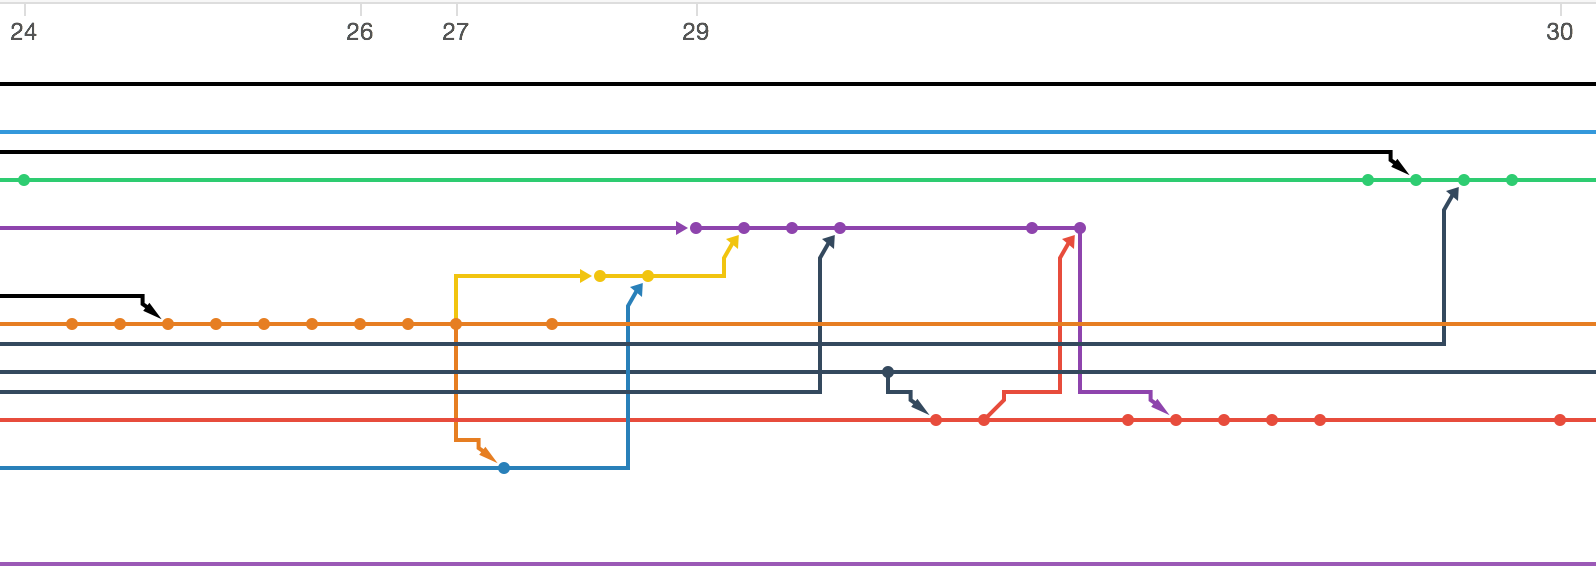
\includegraphics[scale=0.5]{diagram2}
\caption{Git diagram 2}
\label{figure:diagram2}
\end{figure} 

%----------------------------------------------------------------------------
\section{Continuous Deployment}
\label{deployment}

An unforeseen benefit of using the combination of Git and Github was the ease by which the system could be deployed. Two instances of the project were hosted on Heroku, a platform for hosting dynamically scalable web applications. The first instance hosted the code held within the master branch of the Git repository. The second instance ran the code present in the “beta” branch of the project.

An extension to the Heroku platform called Codeship was used to ease the deployment of new builds. Codeship is a continuous deployment platform which was configured so that any changes to the master branch or the beta branch were automatically built and deployed to their respective live websites.


%============================================================================
\chapter{Implementation}
\label{impl}

Once the requirements for the system had been identified and the way the team was to organise itself had been formalised implementation of the system could begin.


%----------------------------------------------------------------------------
\section{Model Implementation}
\label{modelImpl}

The system implementation began with the creation of a framework from which to build upon.  Models were implemented as identified in the ER diagram \autoref{figure:ERDiagram} using Django’s built in Object Relational Mapper (ORM). During the initial stages of development, these objects were mapped to a SQLite schema, but as development progressed, the PostgreSQL database management system was used instead.


\begin{figure}[ht]
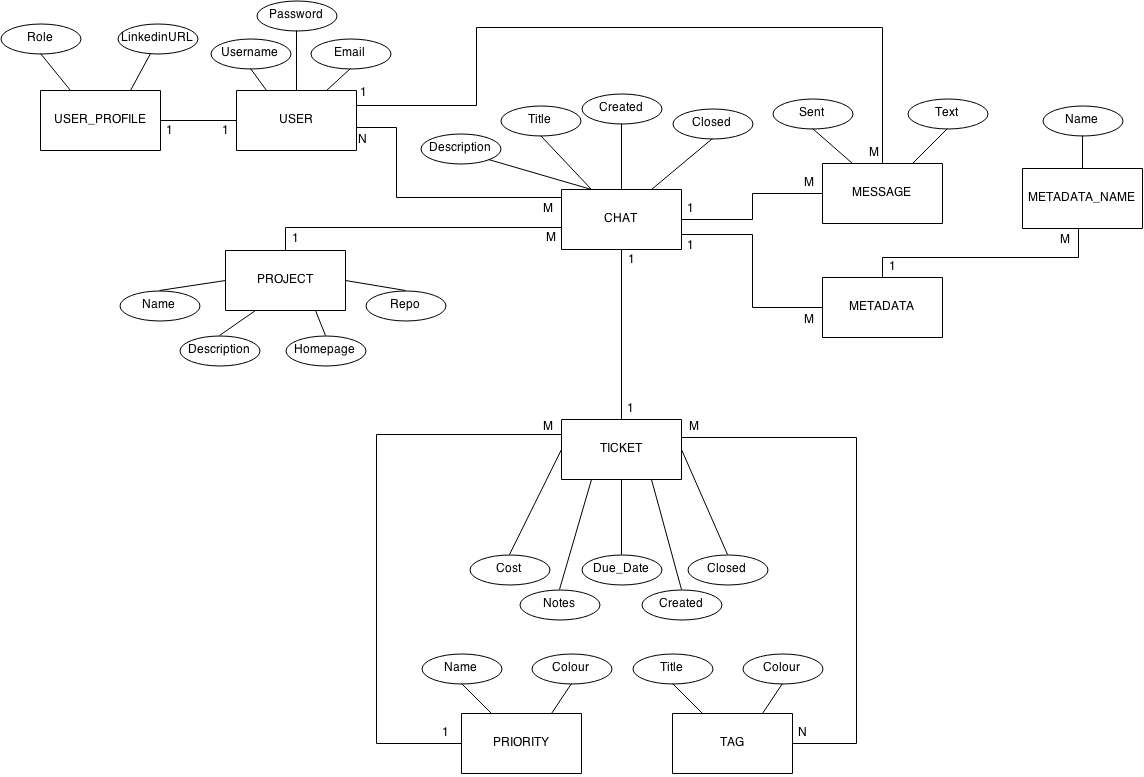
\includegraphics[scale=0.35]{newERdiagram}
\caption{Final ER Diagram}
\label{figure:ERDiagram}
\end{figure}
%----------------------------------------------------------------------------
\section{User Interface}
\label{userInterface}

Due to the system being a web application, the main technologies used in the creation of the user interface were HTML5 and CSS3, as is standard in the vast majority of web based software. 

Twitter’s Bootstrap library was used to manage the layout of web pages, and to improve compatibility with mobile devices. The intuitive grid layout system provided by this library greatly improved the rate at which the UI was developed, since it minimised the extent to which the team had to rely on custom CSS rules.

To accommodate the requirement that the application be more reactive to user interaction, the JQuery Javascript library was used. JQuery assists almost every element of the application, from displaying new messages on the screen, to highlighting selected issues. 

Perhaps the most important feature of the JQuery library used to make the website more responsive was Ajax (Asynchronous Javascript and XML). Ajax provides the ability to reload only small portions of the screen when required, rather than reloading the entire page and sending multiple requests for objects that have already been transferred. Ajax is the basis for several features of the application that would otherwise respond slowly, such as the search and sort features.
%----------------------------------------------------------------------------
\section{Messaging System}
\label{messagingSystem}

The instant messaging aspect of the project was implemented using a Javascript library and backend service called Firebase. An alternative option considered by the team was to implement a server side mechanism for handling messaging using the WebSocket protocol. However, several disadvantages to this approach were found on investigation:

\begin{itemize}
\item The default Django web server relies on the Web Server Gateway Interface (WSGI) for handling communication between the server and the framework. Due to the request handling mechanism employed by WSGI, it is not possible to support long term connections through the likes of WebSockets, and so an additional server which provides support for the WebSocket protocol would have to be set up to achieve the required functionality.
\item The WebSocket protocol is extremely complex in comparison to the Firebase library, and so it would have been difficult to produce a working system within the time constraints of the project.
\end{itemize}

Another option which was considered was working within the constraints of the Django framework. Creating an instant messaging system within Django would require using an inefficient method such as asynchronous polling, in which the client repeatedly asks the server if a new message has been sent.

The decision to use Firebase was not without its drawbacks:
\begin{itemize}
\item There is an overhead in ensuring that the data in the external storage provided by Firebase remains consistent with the data held within the relational database.
\item Employing a third party storage service added an additional point of failure to the system. On several occasions throughout development, the Firebase API became unavailable, leaving the application unusable for a short period of time.
\item Each member of the team had to understand the API exported by Firebase. Consequently, the project uses two REST APIs for communication with the server side rather than one, increasing the complexity of the design. The Firebase API also proved difficult to work at times, with simple queries departing from the well understood semantics of SQL.
\end{itemize}

In general, the use of an external service to implement the messaging system greatly improved the rate of development of the project and allowed the team to focus on other aspects of the system, which may not have been possible using one of the other options.

%----------------------------------------------------------------------------
\section{Rest API}
\label{restApi}

An Django plugin known as TastyPie was used to convert the models that were previously defined into endpoints that the client can call to request data from the database. After quick initial configuration of the plugin, specified portions of the database schema were available to the client side of the application. 

TODO: write more here
%----------------------------------------------------------------------------
\section{Prototype}
\label{prototype}


A prototype was prepared for demonstration after ten weeks. The interface was simple but fully functional (figure - screenshot of the demonstration). The system had basic functionalities such as: 

\begin{itemize}
\item User registration and login
\item Project creation
\item Creation of independent conversations (tickets)
\item Ability to open and close conversations
\end{itemize}

The aim of the prototype development was to create a basic framework to display, which could then be build upon as opposed to implementing multiple user stories, resulting in a fragmented program with many isolated features but no overall functionality.  The resultant product therefore had a large amount of unseen ‘groundwork’ added and thus while it did not immediately appear as if a lot of work had been completed, allowed new features to be easily implemented as the project progressed. 

%----------------------------------------------------------------------------
\section{Metadata}
\label{metadata}

Notes, due date, cost, assignee, tag, priority.

%----------------------------------------------------------------------------
\section{Statistics}
\label{statistics}

Three graphs were implemented to show a proof-of-concept of how visually representing information would enhance a user’s understanding of their project. 
All visualisations were implemented as simple bar charts. It was found that, in all three cases, the data being displayed was a mapping of ordinal data and quantitative value. Users’ familiarity with bar carts made them an obvious choice for representing the site’s data. 
The graphs provided were:

\begin{itemize}
\item Messages sent per user in a conversation
\item Messages sent per user in a project
\item Messages contained in each conversation in a project
\end{itemize}

These graphs were intended to show user participation and chat activity in a way that would allow an observer to judge the importance of different chats within the system, and to see the contributions a user was making on both a project level and within specific tickets (here conversations) they were working on.

%----------------------------------------------------------------------------
\section{Dogfooding}
\label{dog}
At this point in the implementation the team began using the tool to manage development, ... 


%----------------------------------------------------------------------------
\section{Notifications}
\label{notifications}


%----------------------------------------------------------------------------
\section{Saved Messages}
\label{savedMessages}

Make sure we mention dogfeeding at some point here.

%============================================================================
\chapter{Evaluation}
\label{evaluation}

In this section we should discuss what we did, did it achieve the intended objective, what could be done better, 
future developments and things that were unable to achieve.

An area of potential future development could be integration with the continuous integration system Jenkins.  This could be implemented through treating Jenkins as a user who would automatically create a ticket based on each build.  It could also automatically create a high priority ticket when a build fails, and tag the relevant developers.  This expansion would be possible due to Jenkins plugin based structure, whereby it is designed to be extended as necessary.

Another potential addition could be linking to Git and other source control platforms. Often, these systems support tickets and issue control to some degree; 

%----------------------------------------------------------------------------
\section{Dogfooding}
\label{dogfooding}


%----------------------------------------------------------------------------
\section{External Evaluation}
\label{externalEvaluation}


%----------------------------------------------------------------------------
\section{Retrospective}
\label{retrospective}


%============================================================================
\chapter{Conclusion}
\label{conclusion}


%----------------------------------------------------------------------------
\section{Future Goals}
\label{futureGoals}


%============================================================================
% \bibliographystyle{plain}
% \bibliography{example}
\end{document}
